\documentclass{standalone}
\usepackage{tikz}
\usepackage{pgfplots}
\pgfplotsset{compat=1.18}

\begin{document}
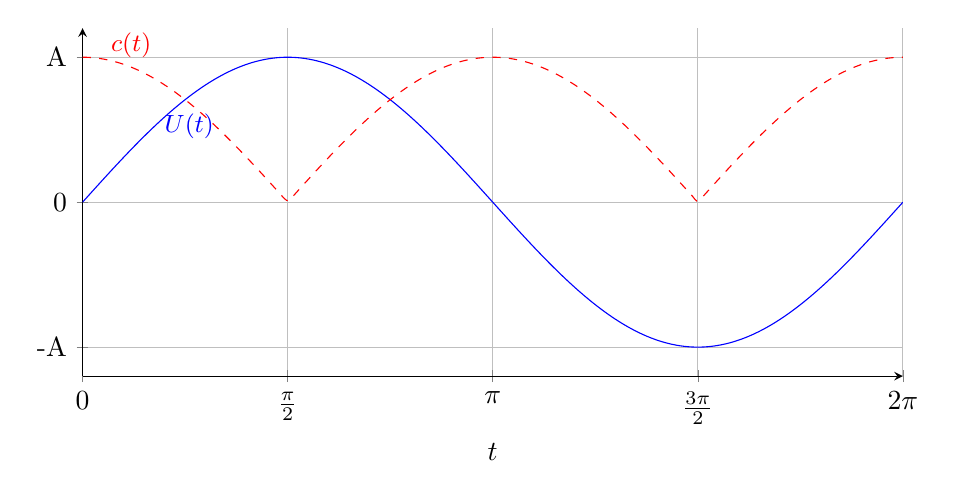
\begin{tikzpicture}
    \begin{axis}[
        width=12cm,
        height=6cm,
        xlabel={$t$},
        ylabel={},
        grid=major,
        xmin=0, xmax=6.28318,
        ymin=-1.2, ymax=1.2,
        xtick={0, 1.5708, 3.14159, 4.71239, 6.28318},
        xticklabels={$0$, $\frac{\pi}{2}$, $\pi$, $\frac{3\pi}{2}$, $2\pi$},
        ytick={-1, 0, 1},
        yticklabels={-A, 0, A},
        axis lines=left
    ]
        \addplot[blue, domain=0:2*pi, samples=200, smooth] {sin(deg(x))} node[right, pos=0.1, font=\small] {$U(t)$};
        \addplot[red, domain=0:2*pi, samples=200, smooth, dashed] {abs(cos(deg(x)))} node[above, pos=0.05, font=\small] {$c(t)$};
    \end{axis}
\end{tikzpicture}
\end{document}
